% Options for packages loaded elsewhere
\PassOptionsToPackage{unicode}{hyperref}
\PassOptionsToPackage{hyphens}{url}
%
\documentclass[
]{article}
\usepackage{amsmath,amssymb}
\usepackage{lmodern}
\usepackage{iftex}
\ifPDFTeX
  \usepackage[T1]{fontenc}
  \usepackage[utf8]{inputenc}
  \usepackage{textcomp} % provide euro and other symbols
\else % if luatex or xetex
  \usepackage{unicode-math}
  \defaultfontfeatures{Scale=MatchLowercase}
  \defaultfontfeatures[\rmfamily]{Ligatures=TeX,Scale=1}
\fi
% Use upquote if available, for straight quotes in verbatim environments
\IfFileExists{upquote.sty}{\usepackage{upquote}}{}
\IfFileExists{microtype.sty}{% use microtype if available
  \usepackage[]{microtype}
  \UseMicrotypeSet[protrusion]{basicmath} % disable protrusion for tt fonts
}{}
\makeatletter
\@ifundefined{KOMAClassName}{% if non-KOMA class
  \IfFileExists{parskip.sty}{%
    \usepackage{parskip}
  }{% else
    \setlength{\parindent}{0pt}
    \setlength{\parskip}{6pt plus 2pt minus 1pt}}
}{% if KOMA class
  \KOMAoptions{parskip=half}}
\makeatother
\usepackage{xcolor}
\usepackage[margin=1in]{geometry}
\usepackage{color}
\usepackage{fancyvrb}
\newcommand{\VerbBar}{|}
\newcommand{\VERB}{\Verb[commandchars=\\\{\}]}
\DefineVerbatimEnvironment{Highlighting}{Verbatim}{commandchars=\\\{\}}
% Add ',fontsize=\small' for more characters per line
\usepackage{framed}
\definecolor{shadecolor}{RGB}{248,248,248}
\newenvironment{Shaded}{\begin{snugshade}}{\end{snugshade}}
\newcommand{\AlertTok}[1]{\textcolor[rgb]{0.94,0.16,0.16}{#1}}
\newcommand{\AnnotationTok}[1]{\textcolor[rgb]{0.56,0.35,0.01}{\textbf{\textit{#1}}}}
\newcommand{\AttributeTok}[1]{\textcolor[rgb]{0.77,0.63,0.00}{#1}}
\newcommand{\BaseNTok}[1]{\textcolor[rgb]{0.00,0.00,0.81}{#1}}
\newcommand{\BuiltInTok}[1]{#1}
\newcommand{\CharTok}[1]{\textcolor[rgb]{0.31,0.60,0.02}{#1}}
\newcommand{\CommentTok}[1]{\textcolor[rgb]{0.56,0.35,0.01}{\textit{#1}}}
\newcommand{\CommentVarTok}[1]{\textcolor[rgb]{0.56,0.35,0.01}{\textbf{\textit{#1}}}}
\newcommand{\ConstantTok}[1]{\textcolor[rgb]{0.00,0.00,0.00}{#1}}
\newcommand{\ControlFlowTok}[1]{\textcolor[rgb]{0.13,0.29,0.53}{\textbf{#1}}}
\newcommand{\DataTypeTok}[1]{\textcolor[rgb]{0.13,0.29,0.53}{#1}}
\newcommand{\DecValTok}[1]{\textcolor[rgb]{0.00,0.00,0.81}{#1}}
\newcommand{\DocumentationTok}[1]{\textcolor[rgb]{0.56,0.35,0.01}{\textbf{\textit{#1}}}}
\newcommand{\ErrorTok}[1]{\textcolor[rgb]{0.64,0.00,0.00}{\textbf{#1}}}
\newcommand{\ExtensionTok}[1]{#1}
\newcommand{\FloatTok}[1]{\textcolor[rgb]{0.00,0.00,0.81}{#1}}
\newcommand{\FunctionTok}[1]{\textcolor[rgb]{0.00,0.00,0.00}{#1}}
\newcommand{\ImportTok}[1]{#1}
\newcommand{\InformationTok}[1]{\textcolor[rgb]{0.56,0.35,0.01}{\textbf{\textit{#1}}}}
\newcommand{\KeywordTok}[1]{\textcolor[rgb]{0.13,0.29,0.53}{\textbf{#1}}}
\newcommand{\NormalTok}[1]{#1}
\newcommand{\OperatorTok}[1]{\textcolor[rgb]{0.81,0.36,0.00}{\textbf{#1}}}
\newcommand{\OtherTok}[1]{\textcolor[rgb]{0.56,0.35,0.01}{#1}}
\newcommand{\PreprocessorTok}[1]{\textcolor[rgb]{0.56,0.35,0.01}{\textit{#1}}}
\newcommand{\RegionMarkerTok}[1]{#1}
\newcommand{\SpecialCharTok}[1]{\textcolor[rgb]{0.00,0.00,0.00}{#1}}
\newcommand{\SpecialStringTok}[1]{\textcolor[rgb]{0.31,0.60,0.02}{#1}}
\newcommand{\StringTok}[1]{\textcolor[rgb]{0.31,0.60,0.02}{#1}}
\newcommand{\VariableTok}[1]{\textcolor[rgb]{0.00,0.00,0.00}{#1}}
\newcommand{\VerbatimStringTok}[1]{\textcolor[rgb]{0.31,0.60,0.02}{#1}}
\newcommand{\WarningTok}[1]{\textcolor[rgb]{0.56,0.35,0.01}{\textbf{\textit{#1}}}}
\usepackage{graphicx}
\makeatletter
\def\maxwidth{\ifdim\Gin@nat@width>\linewidth\linewidth\else\Gin@nat@width\fi}
\def\maxheight{\ifdim\Gin@nat@height>\textheight\textheight\else\Gin@nat@height\fi}
\makeatother
% Scale images if necessary, so that they will not overflow the page
% margins by default, and it is still possible to overwrite the defaults
% using explicit options in \includegraphics[width, height, ...]{}
\setkeys{Gin}{width=\maxwidth,height=\maxheight,keepaspectratio}
% Set default figure placement to htbp
\makeatletter
\def\fps@figure{htbp}
\makeatother
\setlength{\emergencystretch}{3em} % prevent overfull lines
\providecommand{\tightlist}{%
  \setlength{\itemsep}{0pt}\setlength{\parskip}{0pt}}
\setcounter{secnumdepth}{-\maxdimen} % remove section numbering
\ifLuaTeX
  \usepackage{selnolig}  % disable illegal ligatures
\fi
\IfFileExists{bookmark.sty}{\usepackage{bookmark}}{\usepackage{hyperref}}
\IfFileExists{xurl.sty}{\usepackage{xurl}}{} % add URL line breaks if available
\urlstyle{same} % disable monospaced font for URLs
\hypersetup{
  pdftitle={MATHS 7107 Data Taming},
  pdfauthor={Chang Dong},
  hidelinks,
  pdfcreator={LaTeX via pandoc}}

\title{MATHS 7107 Data Taming}
\author{Chang Dong}
\date{2023-03-31}

\begin{document}
\maketitle

\hypertarget{part-1}{%
\subsection{Part 1}\label{part-1}}

First we will start by looking at how to measure a model using
yardstick. We will fit a regression model, and also a classification
model to the penguins dataset and then have a look at assessing them.

\hypertarget{load-the-data-and-required-packages}{%
\subsection{Load the data and required
packages}\label{load-the-data-and-required-packages}}

\begin{Shaded}
\begin{Highlighting}[]
\NormalTok{pacman}\SpecialCharTok{::}\FunctionTok{p\_load}\NormalTok{(tidyverse, tidymodels,palmerpenguins,harrypotter)}

\FunctionTok{data}\NormalTok{(}\StringTok{"penguins"}\NormalTok{, }\AttributeTok{package =} \StringTok{"palmerpenguins"}\NormalTok{)}
\end{Highlighting}
\end{Shaded}

\hypertarget{create-the-models}{%
\subsection{Create the models}\label{create-the-models}}

\begin{Shaded}
\begin{Highlighting}[]
\NormalTok{penguin\_M1 }\OtherTok{\textless{}{-}} \FunctionTok{workflow}\NormalTok{() }\SpecialCharTok{\%\textgreater{}\%} 
  \FunctionTok{add\_formula}\NormalTok{(flipper\_length\_mm }\SpecialCharTok{\textasciitilde{}}\NormalTok{ body\_mass\_g) }\SpecialCharTok{\%\textgreater{}\%} 
  \FunctionTok{add\_model}\NormalTok{( }\FunctionTok{linear\_reg}\NormalTok{() }\SpecialCharTok{\%\textgreater{}\%} \FunctionTok{set\_engine}\NormalTok{(}\StringTok{"lm"}\NormalTok{) ) }\SpecialCharTok{\%\textgreater{}\%} 
  \FunctionTok{fit}\NormalTok{(penguins) }
\NormalTok{penguin\_M1}
\end{Highlighting}
\end{Shaded}

\begin{verbatim}
## == Workflow [trained] ==========================================================
## Preprocessor: Formula
## Model: linear_reg()
## 
## -- Preprocessor ----------------------------------------------------------------
## flipper_length_mm ~ body_mass_g
## 
## -- Model -----------------------------------------------------------------------
## 
## Call:
## stats::lm(formula = ..y ~ ., data = data)
## 
## Coefficients:
## (Intercept)  body_mass_g  
##   136.72956      0.01528
\end{verbatim}

\begin{Shaded}
\begin{Highlighting}[]
\NormalTok{penguin\_M2 }\OtherTok{\textless{}{-}} \FunctionTok{workflow}\NormalTok{() }\SpecialCharTok{\%\textgreater{}\%} 
  \FunctionTok{add\_formula}\NormalTok{(sex }\SpecialCharTok{\textasciitilde{}}\NormalTok{ body\_mass\_g) }\SpecialCharTok{\%\textgreater{}\%} 
  \FunctionTok{add\_model}\NormalTok{(}
    \FunctionTok{logistic\_reg}\NormalTok{() }\SpecialCharTok{\%\textgreater{}\%} 
      \FunctionTok{set\_engine}\NormalTok{(}\StringTok{"glm"}\NormalTok{)}
\NormalTok{  ) }\SpecialCharTok{\%\textgreater{}\%}
  \FunctionTok{fit}\NormalTok{(penguins) }
\NormalTok{penguin\_M2}
\end{Highlighting}
\end{Shaded}

\begin{verbatim}
## == Workflow [trained] ==========================================================
## Preprocessor: Formula
## Model: logistic_reg()
## 
## -- Preprocessor ----------------------------------------------------------------
## sex ~ body_mass_g
## 
## -- Model -----------------------------------------------------------------------
## 
## Call:  stats::glm(formula = ..y ~ ., family = stats::binomial, data = data)
## 
## Coefficients:
## (Intercept)  body_mass_g  
##    -5.16254      0.00124  
## 
## Degrees of Freedom: 332 Total (i.e. Null);  331 Residual
##   (11 observations deleted due to missingness)
## Null Deviance:       461.6 
## Residual Deviance: 396.6     AIC: 400.6
\end{verbatim}

\hypertarget{question-for-model-1-what-are-the-response-variable-and-the-predictors.}{%
\paragraph{Question: For model 1, what are the response variable and the
predictors.}\label{question-for-model-1-what-are-the-response-variable-and-the-predictors.}}

\begin{Shaded}
\begin{Highlighting}[]
\CommentTok{\# The response variable is flipper length and the predictor is body mass.}
\end{Highlighting}
\end{Shaded}

\hypertarget{question-for-model-2-what-are-the-response-variable-and-the-predictors.}{%
\paragraph{Question: For model 2, what are the response variable and the
predictors.}\label{question-for-model-2-what-are-the-response-variable-and-the-predictors.}}

\begin{Shaded}
\begin{Highlighting}[]
\CommentTok{\# The response variable is sex and the predictor is body mass.}
\end{Highlighting}
\end{Shaded}

\hypertarget{getting-prediction}{%
\subsection{Getting prediction}\label{getting-prediction}}

For yardstick, we will need predicted values, we obtain that using the
predict() function. Here I will add a variety of predictions to the
original dataset.

\begin{Shaded}
\begin{Highlighting}[]
\NormalTok{penguins\_pred }\OtherTok{\textless{}{-}}\NormalTok{ penguins }\SpecialCharTok{\%\textgreater{}\%} 
  \FunctionTok{bind\_cols}\NormalTok{( }\FunctionTok{predict}\NormalTok{(penguin\_M1, penguins), }
             \FunctionTok{predict}\NormalTok{(penguin\_M2, penguins), }
             \FunctionTok{predict}\NormalTok{(penguin\_M2, penguins,}\AttributeTok{type =} \StringTok{"prob"}\NormalTok{),}
\NormalTok{            ) }\SpecialCharTok{\%\textgreater{}\%} 
  \FunctionTok{select}\NormalTok{(sex, flipper\_length\_mm,}\FunctionTok{starts\_with}\NormalTok{(}\StringTok{".pred"}\NormalTok{)) }
\NormalTok{penguins\_pred}
\end{Highlighting}
\end{Shaded}

\begin{verbatim}
## # A tibble: 344 x 6
##    sex    flipper_length_mm .pred .pred_class .pred_female .pred_male
##    <fct>              <int> <dbl> <fct>              <dbl>      <dbl>
##  1 male                 181  194. female             0.626      0.374
##  2 female               186  195. female             0.611      0.389
##  3 female               195  186. female             0.756      0.244
##  4 <NA>                  NA   NA  <NA>              NA         NA    
##  5 female               193  189. female             0.708      0.292
##  6 male                 190  192. female             0.654      0.346
##  7 female               181  192. female             0.661      0.339
##  8 male                 195  208. male               0.347      0.653
##  9 <NA>                 193  190. female             0.701      0.299
## 10 <NA>                 190  202. male               0.473      0.527
## # ... with 334 more rows
\end{verbatim}

\hypertarget{question-what-is-the-predicted-flipper-length-for-the-first-penguin}{%
\paragraph{Question: What is the predicted flipper length for the first
penguin?}\label{question-what-is-the-predicted-flipper-length-for-the-first-penguin}}

\begin{Shaded}
\begin{Highlighting}[]
\CommentTok{\# The predicted flipper length is 194mm}
\end{Highlighting}
\end{Shaded}

\#\#\#\#Question: What is the predicted probability of being male for
the first penguin?

\begin{Shaded}
\begin{Highlighting}[]
\CommentTok{\# The predicted prob is 0.374.}
\end{Highlighting}
\end{Shaded}

\hypertarget{categorical-metrics}{%
\subsubsection{Categorical metrics}\label{categorical-metrics}}

For most of the metrics, we will use the hard classification for the
categorical variable as given by .pred\_class. We can get the confusion
matrix:

\begin{Shaded}
\begin{Highlighting}[]
\NormalTok{penguins\_pred }\SpecialCharTok{\%\textgreater{}\%} \FunctionTok{conf\_mat}\NormalTok{( }\AttributeTok{truth =}\NormalTok{ sex, }\AttributeTok{estimate =}\NormalTok{ .pred\_class )}
\end{Highlighting}
\end{Shaded}

\begin{verbatim}
##           Truth
## Prediction female male
##     female    109   74
##     male       56   94
\end{verbatim}

\hypertarget{question-how-many-of-the-females-we-incorrectly-predicted-as-male}{%
\paragraph{Question: How many of the females, we incorrectly predicted
as
male?}\label{question-how-many-of-the-females-we-incorrectly-predicted-as-male}}

\begin{Shaded}
\begin{Highlighting}[]
\CommentTok{\# 56 of the female penguins were incorrectly identified as male}
\end{Highlighting}
\end{Shaded}

We can get the sensitivity as follows:

\begin{Shaded}
\begin{Highlighting}[]
\NormalTok{penguins\_pred }\SpecialCharTok{\%\textgreater{}\%} \FunctionTok{sens}\NormalTok{( }\AttributeTok{truth =}\NormalTok{ sex, }\AttributeTok{estimate =}\NormalTok{ .pred\_class )}
\end{Highlighting}
\end{Shaded}

\begin{verbatim}
## # A tibble: 1 x 3
##   .metric .estimator .estimate
##   <chr>   <chr>          <dbl>
## 1 sens    binary         0.661
\end{verbatim}

\hypertarget{question-what-is-the-specificity}{%
\paragraph{Question: What is the
specificity?}\label{question-what-is-the-specificity}}

We can obtain a set of the metrics as follows:

\begin{Shaded}
\begin{Highlighting}[]
\NormalTok{categorical\_metrics }\OtherTok{\textless{}{-}} \FunctionTok{metric\_set}\NormalTok{(sens, spec, precision, recall) }
\NormalTok{penguins\_pred }\SpecialCharTok{\%\textgreater{}\%} 
  \FunctionTok{categorical\_metrics}\NormalTok{( }\AttributeTok{truth =}\NormalTok{ sex, }\AttributeTok{estimate =}\NormalTok{ .pred\_class )}
\end{Highlighting}
\end{Shaded}

\begin{verbatim}
## # A tibble: 4 x 3
##   .metric   .estimator .estimate
##   <chr>     <chr>          <dbl>
## 1 sens      binary         0.661
## 2 spec      binary         0.560
## 3 precision binary         0.596
## 4 recall    binary         0.661
\end{verbatim}

\begin{Shaded}
\begin{Highlighting}[]
\CommentTok{\# The specificity is 0.560}
\end{Highlighting}
\end{Shaded}

\hypertarget{question-what-is-the-precision}{%
\paragraph{Question: What is the
precision?}\label{question-what-is-the-precision}}

\begin{Shaded}
\begin{Highlighting}[]
\CommentTok{\# The precision is 0.596}
\end{Highlighting}
\end{Shaded}

We can plot the ROC curve using ggplot2, or quickly using autoplot()

\begin{Shaded}
\begin{Highlighting}[]
\NormalTok{penguins\_pred }\SpecialCharTok{\%\textgreater{}\%} 
  \FunctionTok{roc\_curve}\NormalTok{( }\AttributeTok{truth =}\NormalTok{ sex, }\AttributeTok{estimate =}\NormalTok{ .pred\_female ) }\SpecialCharTok{\%\textgreater{}\%} 
  \FunctionTok{autoplot}\NormalTok{()}
\end{Highlighting}
\end{Shaded}

\begin{verbatim}
## Warning: Returning more (or less) than 1 row per `summarise()` group was deprecated in
## dplyr 1.1.0.
## i Please use `reframe()` instead.
## i When switching from `summarise()` to `reframe()`, remember that `reframe()`
##   always returns an ungrouped data frame and adjust accordingly.
## i The deprecated feature was likely used in the yardstick package.
##   Please report the issue at <]8;;https://github.com/tidymodels/yardstick/issueshttps://github.com/tidymodels/yardstick/issues]8;;>.
\end{verbatim}

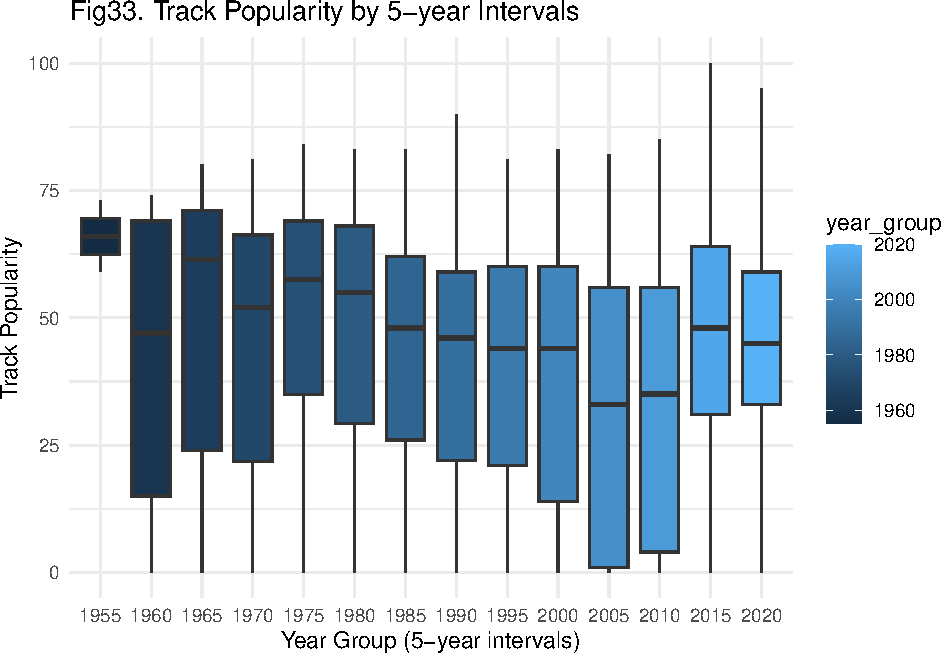
\includegraphics{week9_files/figure-latex/unnamed-chunk-15-1.pdf}

\hypertarget{question-what-is-the-auc-for-m2}{%
\paragraph{Question: What is the AUC for
M2?}\label{question-what-is-the-auc-for-m2}}

We can obtain this as follows:

\begin{Shaded}
\begin{Highlighting}[]
\NormalTok{penguins\_pred }\SpecialCharTok{\%\textgreater{}\%} \FunctionTok{roc\_auc}\NormalTok{( }\AttributeTok{truth =}\NormalTok{ sex, }\AttributeTok{estimate =}\NormalTok{ .pred\_female )}
\end{Highlighting}
\end{Shaded}

\begin{verbatim}
## # A tibble: 1 x 3
##   .metric .estimator .estimate
##   <chr>   <chr>          <dbl>
## 1 roc_auc binary         0.752
\end{verbatim}

\begin{Shaded}
\begin{Highlighting}[]
\CommentTok{\# The AUC is 0.752}
\end{Highlighting}
\end{Shaded}

\hypertarget{part-2}{%
\subsection{Part 2}\label{part-2}}

Now we are going to show how to split your data into folds for
cross-validation. We will use then use cross-validation to get a more
accurate measure of how well our models fit.

\hypertarget{load-and-split-the-data}{%
\subsection{Load and split the data}\label{load-and-split-the-data}}

Back to the penguins - why would you not?

First we are going to split our dataset into a test data to save for the
very end, and the training data.

\begin{Shaded}
\begin{Highlighting}[]
\FunctionTok{set.seed}\NormalTok{(}\DecValTok{2021}\NormalTok{) }
\NormalTok{penguin\_split }\OtherTok{\textless{}{-}} \FunctionTok{initial\_split}\NormalTok{(penguins) }
\NormalTok{penguin\_split}
\end{Highlighting}
\end{Shaded}

\begin{verbatim}
## <Training/Testing/Total>
## <258/86/344>
\end{verbatim}

\begin{Shaded}
\begin{Highlighting}[]
\NormalTok{penguins\_train }\OtherTok{\textless{}{-}} \FunctionTok{training}\NormalTok{(penguin\_split) }
\NormalTok{penguins\_test }\OtherTok{\textless{}{-}} \FunctionTok{testing}\NormalTok{(penguin\_split)}
\end{Highlighting}
\end{Shaded}

\hypertarget{question-how-many-penguins-in-the-test-dataset}{%
\paragraph{Question: How many penguins in the test
dataset?}\label{question-how-many-penguins-in-the-test-dataset}}

\begin{Shaded}
\begin{Highlighting}[]
\CommentTok{\# There are 86 penguins in the test dataset.}
\end{Highlighting}
\end{Shaded}

Now we are going to split our training dataset into folds:

\begin{Shaded}
\begin{Highlighting}[]
\NormalTok{penguin\_CV }\OtherTok{\textless{}{-}} \FunctionTok{vfold\_cv}\NormalTok{(penguins\_train) }
\NormalTok{penguin\_CV}
\end{Highlighting}
\end{Shaded}

\begin{verbatim}
## #  10-fold cross-validation 
## # A tibble: 10 x 2
##    splits           id    
##    <list>           <chr> 
##  1 <split [232/26]> Fold01
##  2 <split [232/26]> Fold02
##  3 <split [232/26]> Fold03
##  4 <split [232/26]> Fold04
##  5 <split [232/26]> Fold05
##  6 <split [232/26]> Fold06
##  7 <split [232/26]> Fold07
##  8 <split [232/26]> Fold08
##  9 <split [233/25]> Fold09
## 10 <split [233/25]> Fold10
\end{verbatim}

\hypertarget{question-how-many-folds-are-produced}{%
\paragraph{Question: How many folds are
produced?}\label{question-how-many-folds-are-produced}}

\begin{Shaded}
\begin{Highlighting}[]
\CommentTok{\# In total there are 10 folds. This is the default.}
\end{Highlighting}
\end{Shaded}

\hypertarget{fit-models-and-get-measures}{%
\subsubsection{Fit models and get
measures}\label{fit-models-and-get-measures}}

We will set up two workflows - one regression, and one classification.
For linear regression:

\begin{Shaded}
\begin{Highlighting}[]
\NormalTok{linear\_model }\OtherTok{\textless{}{-}} \FunctionTok{linear\_reg}\NormalTok{() }\SpecialCharTok{\%\textgreater{}\%} 
  \FunctionTok{set\_engine}\NormalTok{(}\StringTok{"lm"}\NormalTok{)}

\NormalTok{penguin\_linear\_workflow }\OtherTok{\textless{}{-}} \FunctionTok{workflow}\NormalTok{() }\SpecialCharTok{\%\textgreater{}\%} 
  \FunctionTok{add\_model}\NormalTok{(linear\_model) }\SpecialCharTok{\%\textgreater{}\%} 
  \FunctionTok{add\_formula}\NormalTok{(bill\_length\_mm }\SpecialCharTok{\textasciitilde{}}\NormalTok{ body\_mass\_g)}
\end{Highlighting}
\end{Shaded}

For logistic regression:

\begin{Shaded}
\begin{Highlighting}[]
\NormalTok{logistic\_model }\OtherTok{\textless{}{-}} \FunctionTok{logistic\_reg}\NormalTok{() }\SpecialCharTok{\%\textgreater{}\%} 
  \FunctionTok{set\_engine}\NormalTok{(}\StringTok{"glm"}\NormalTok{)}

\NormalTok{penguin\_logistic\_workflow }\OtherTok{\textless{}{-}} \FunctionTok{workflow}\NormalTok{() }\SpecialCharTok{\%\textgreater{}\%} 
  \FunctionTok{add\_model}\NormalTok{(logistic\_model) }\SpecialCharTok{\%\textgreater{}\%} 
  \FunctionTok{add\_formula}\NormalTok{(sex }\SpecialCharTok{\textasciitilde{}}\NormalTok{ body\_mass\_g)}
\end{Highlighting}
\end{Shaded}

The key function is fit\_resamples. This function will take a workflow,
and folds and preform multiple fits. It fits the model to the CV
training dataset, and then fits the model to the test CV and grabs some
metrics.

\begin{Shaded}
\begin{Highlighting}[]
\NormalTok{penguin\_linear\_resamples }\OtherTok{\textless{}{-}} \FunctionTok{fit\_resamples}\NormalTok{( }
\NormalTok{  penguin\_linear\_workflow, }
  \AttributeTok{resamples =}\NormalTok{ penguin\_CV ) }
\NormalTok{penguin\_linear\_resamples}
\end{Highlighting}
\end{Shaded}

\begin{verbatim}
## # Resampling results
## # 10-fold cross-validation 
## # A tibble: 10 x 4
##    splits           id     .metrics         .notes          
##    <list>           <chr>  <list>           <list>          
##  1 <split [232/26]> Fold01 <tibble [2 x 4]> <tibble [0 x 3]>
##  2 <split [232/26]> Fold02 <tibble [2 x 4]> <tibble [0 x 3]>
##  3 <split [232/26]> Fold03 <tibble [2 x 4]> <tibble [0 x 3]>
##  4 <split [232/26]> Fold04 <tibble [2 x 4]> <tibble [0 x 3]>
##  5 <split [232/26]> Fold05 <tibble [2 x 4]> <tibble [0 x 3]>
##  6 <split [232/26]> Fold06 <tibble [2 x 4]> <tibble [0 x 3]>
##  7 <split [232/26]> Fold07 <tibble [2 x 4]> <tibble [0 x 3]>
##  8 <split [232/26]> Fold08 <tibble [2 x 4]> <tibble [0 x 3]>
##  9 <split [233/25]> Fold09 <tibble [2 x 4]> <tibble [0 x 3]>
## 10 <split [233/25]> Fold10 <tibble [2 x 4]> <tibble [0 x 3]>
\end{verbatim}

If we want to keep the prediction values on the CV test set, then we
use:

\begin{Shaded}
\begin{Highlighting}[]
\NormalTok{control }\OtherTok{=} \FunctionTok{control\_resamples}\NormalTok{(}\AttributeTok{save\_pred =} \ConstantTok{TRUE}\NormalTok{)}
\end{Highlighting}
\end{Shaded}

Here is an example with the logistic regression.

\begin{Shaded}
\begin{Highlighting}[]
\NormalTok{penguin\_logistic\_resamples }\OtherTok{\textless{}{-}} 
  \FunctionTok{fit\_resamples}\NormalTok{( penguin\_logistic\_workflow, }
                 \AttributeTok{resamples =}\NormalTok{ penguin\_CV, }
                 \AttributeTok{control =} \FunctionTok{control\_resamples}\NormalTok{(}\AttributeTok{save\_pred =} \ConstantTok{TRUE}\NormalTok{)}
\NormalTok{)}
\end{Highlighting}
\end{Shaded}

We can now get the metrics out. Unnest returns all of them, while
collect\_metrics gives us the average:

\begin{Shaded}
\begin{Highlighting}[]
\NormalTok{penguin\_linear\_resamples }\SpecialCharTok{\%\textgreater{}\%} \FunctionTok{unnest}\NormalTok{(.metrics)}
\end{Highlighting}
\end{Shaded}

\begin{verbatim}
## # A tibble: 20 x 7
##    splits           id     .metric .estimator .estimate .config         .notes  
##    <list>           <chr>  <chr>   <chr>          <dbl> <chr>           <list>  
##  1 <split [232/26]> Fold01 rmse    standard       4.41  Preprocessor1_~ <tibble>
##  2 <split [232/26]> Fold01 rsq     standard       0.305 Preprocessor1_~ <tibble>
##  3 <split [232/26]> Fold02 rmse    standard       3.54  Preprocessor1_~ <tibble>
##  4 <split [232/26]> Fold02 rsq     standard       0.594 Preprocessor1_~ <tibble>
##  5 <split [232/26]> Fold03 rmse    standard       3.08  Preprocessor1_~ <tibble>
##  6 <split [232/26]> Fold03 rsq     standard       0.645 Preprocessor1_~ <tibble>
##  7 <split [232/26]> Fold04 rmse    standard       4.67  Preprocessor1_~ <tibble>
##  8 <split [232/26]> Fold04 rsq     standard       0.288 Preprocessor1_~ <tibble>
##  9 <split [232/26]> Fold05 rmse    standard       3.55  Preprocessor1_~ <tibble>
## 10 <split [232/26]> Fold05 rsq     standard       0.535 Preprocessor1_~ <tibble>
## 11 <split [232/26]> Fold06 rmse    standard       4.19  Preprocessor1_~ <tibble>
## 12 <split [232/26]> Fold06 rsq     standard       0.319 Preprocessor1_~ <tibble>
## 13 <split [232/26]> Fold07 rmse    standard       4.59  Preprocessor1_~ <tibble>
## 14 <split [232/26]> Fold07 rsq     standard       0.150 Preprocessor1_~ <tibble>
## 15 <split [232/26]> Fold08 rmse    standard       5.54  Preprocessor1_~ <tibble>
## 16 <split [232/26]> Fold08 rsq     standard       0.206 Preprocessor1_~ <tibble>
## 17 <split [233/25]> Fold09 rmse    standard       5.01  Preprocessor1_~ <tibble>
## 18 <split [233/25]> Fold09 rsq     standard       0.527 Preprocessor1_~ <tibble>
## 19 <split [233/25]> Fold10 rmse    standard       4.40  Preprocessor1_~ <tibble>
## 20 <split [233/25]> Fold10 rsq     standard       0.275 Preprocessor1_~ <tibble>
\end{verbatim}

\begin{Shaded}
\begin{Highlighting}[]
\NormalTok{penguin\_linear\_resamples }\SpecialCharTok{\%\textgreater{}\%} \FunctionTok{collect\_metrics}\NormalTok{()}
\end{Highlighting}
\end{Shaded}

\begin{verbatim}
## # A tibble: 2 x 6
##   .metric .estimator  mean     n std_err .config             
##   <chr>   <chr>      <dbl> <int>   <dbl> <chr>               
## 1 rmse    standard   4.30     10  0.234  Preprocessor1_Model1
## 2 rsq     standard   0.384    10  0.0551 Preprocessor1_Model1
\end{verbatim}

\hypertarget{question-what-is-the-rmse-for-the-first-fold}{%
\paragraph{Question: What is the RMSE for the first
fold?}\label{question-what-is-the-rmse-for-the-first-fold}}

\begin{Shaded}
\begin{Highlighting}[]
\CommentTok{\# The RMSE for the first fold is 4.41.}
\end{Highlighting}
\end{Shaded}

\hypertarget{question-what-is-the-mean-cv-rmse-the-mean-cv-rmse-is-4.30}{%
\paragraph{Question: What is the mean CV RMSE? \# The mean CV RMSE is
4.30}\label{question-what-is-the-mean-cv-rmse-the-mean-cv-rmse-is-4.30}}

You can produce a plot for the logistic regression model as follows:

\begin{Shaded}
\begin{Highlighting}[]
\NormalTok{penguin\_logistic\_resamples }\SpecialCharTok{\%\textgreater{}\%} 
  \FunctionTok{collect\_predictions}\NormalTok{() }\SpecialCharTok{\%\textgreater{}\%} 
  \FunctionTok{group\_by}\NormalTok{(id) }\SpecialCharTok{\%\textgreater{}\%} 
  \FunctionTok{roc\_curve}\NormalTok{(}\AttributeTok{truth =}\NormalTok{ sex, }\AttributeTok{estimate =}\NormalTok{ .pred\_female) }\SpecialCharTok{\%\textgreater{}\%} 
  \FunctionTok{autoplot}\NormalTok{() }\SpecialCharTok{+}
\NormalTok{  harrypotter}\SpecialCharTok{::}\FunctionTok{scale\_color\_hp}\NormalTok{(}\StringTok{"Ravenclaw"}\NormalTok{, }\AttributeTok{discrete =} \ConstantTok{TRUE}\NormalTok{)}
\end{Highlighting}
\end{Shaded}

\includegraphics{week9_files/figure-latex/unnamed-chunk-31-1.pdf}

\hypertarget{compare-to-test}{%
\subsection{Compare to test}\label{compare-to-test}}

Finally, we can get the metrics for the test data we saved at the start
using last\_fit

\begin{Shaded}
\begin{Highlighting}[]
\NormalTok{penguin\_linear\_workflow }\SpecialCharTok{\%\textgreater{}\%} 
  \FunctionTok{last\_fit}\NormalTok{(penguin\_split) }\SpecialCharTok{\%\textgreater{}\%} 
  \FunctionTok{collect\_metrics}\NormalTok{()}
\end{Highlighting}
\end{Shaded}

\begin{verbatim}
## # A tibble: 2 x 4
##   .metric .estimator .estimate .config             
##   <chr>   <chr>          <dbl> <chr>               
## 1 rmse    standard       4.58  Preprocessor1_Model1
## 2 rsq     standard       0.323 Preprocessor1_Model1
\end{verbatim}

\begin{Shaded}
\begin{Highlighting}[]
\NormalTok{penguin\_logistic\_workflow }\SpecialCharTok{\%\textgreater{}\%}
  \FunctionTok{last\_fit}\NormalTok{(penguin\_split) }\SpecialCharTok{\%\textgreater{}\%}
  \FunctionTok{collect\_metrics}\NormalTok{()}
\end{Highlighting}
\end{Shaded}

\begin{verbatim}
## # A tibble: 2 x 4
##   .metric  .estimator .estimate .config             
##   <chr>    <chr>          <dbl> <chr>               
## 1 accuracy binary         0.6   Preprocessor1_Model1
## 2 roc_auc  binary         0.771 Preprocessor1_Model1
\end{verbatim}

\hypertarget{question-what-is-the-test-auc}{%
\paragraph{Question What is the test
AUC?}\label{question-what-is-the-test-auc}}

\begin{Shaded}
\begin{Highlighting}[]
\FloatTok{0.771}
\end{Highlighting}
\end{Shaded}

\begin{verbatim}
## [1] 0.771
\end{verbatim}

\end{document}
